\chapter{Statistical Simulation for Spatial Sampling}

The angle increment was derived in section \ref{sec:spasa} and is presented in equation \ref{eq:angle}. To find a compromise between measurement speed and accuracy a compromise has to be found for the error generated by spatial aliasing. 

\section{Implementation}

The simulation is similar to section \ref{sec:spasa} done with the \ac{AF}, however with a two dimensional rectangular $\sfrac{\lambda}{2}$-element spacing array. This brings the advantage that the array size can easily be adjusted. The \ac{FF}-pattern is computed with the Matlab\texttrademark{} class \textit{phased.URA}. Here also a steering vector, consistent of an azimuth and an elevation angle, to specify which direction the main beam of the array is facing. The sampling of the \ac{FF}-pattern is accomplished by the included \textit{pattern(...)} function.\\
This simulation is mainly developed for \acp{CSSG} and the angle increment is computed by equation \ref{eq:angle}. With the number of elements in $z$ direction $N_z$ and the number of elements in $y$ direction $N_y$ the radii $r_s$ and $r_c$ can be computed as

\begin{equation}
2r_s = \sqrt{\left(N_y-1\right)^2+\left(N_z-1\right)^2}\cdot\frac{\lambda}{2},\quad 2r_c=\left(N_y-1\right)\cdot\frac{\lambda}{2},
\end{equation}

resulting in an angle increment of

\begin{equation}
\Delta\Theta^\prime = \frac{\text{SF}\cdot\text{CrefA}\left(\sfrac{2r_s}{\lambda}\right)\cdot 2}{\sqrt{\left(N_y-1\right)^2+\left(N_z-1\right)^2}}\ ,\quad\Delta\Phi^\prime = \frac{\text{SF}\cdot\text{CrefA}\left(\sfrac{2r_c}{\lambda}\right)\cdot 2}{\left(N_y-1\right)}.
\end{equation}

Whereby \ac{CrefA} is a function of diameter in wavelength, compare figure \ref{fig:crefa}. The number of points on each longitude half circle $N_\Theta$ and on each latitude circle $N_\Phi$ is computed and round up:

\begin{equation}
N_\Theta = \bigg\lceil\frac{\pi}{\Delta\Theta^\prime}\bigg\rceil ; \quad N_\Phi^\prime = \bigg\lceil\frac{2\pi}{\Delta\Phi^\prime}\bigg\rceil
\end{equation}

For more sparse sampling at the poles the \ac{CTF} with a value range of $\text{CTF}=\left[0,1\right]$ is introduced to gain Theta dependent azimuth step size:

\begin{equation}
N_\Phi\left(\Theta\right) = \bigg\lceil\frac{2\pi}{\Delta\Phi^\prime}\left(1-\text{CTF}+\text{CTF}\cdot\cos\right(\Theta\left)\right)\bigg\rceil
\end{equation}

For easier computation $N_\Phi\left(\Theta\right)$ is round to 

\begin{equation}
N_\text{round} = \bigg\lceil \frac{N_\Phi^\prime}{k} \bigg\rceil, \ k \in \mathbb{N}
\end{equation}

and not just to the greater integer. So that the angle increment is

\begin{equation}
\Delta\Theta = \frac{\pi}{N_\Theta} , \quad \Delta\Phi\left(\Theta\right) = \frac{2\pi}{N_\Phi\left(\Theta\right)}.
\end{equation}

With the integers in $N_\text{round}$ the advantage is that a uniform \ac{CSSG} can be sampled and the theta dependent phi can be simulated by discarding every $k$th value in each azimuth circle.

\section{Set Up}

\begin{figure}
  \centering
  \subfigure[PDF]{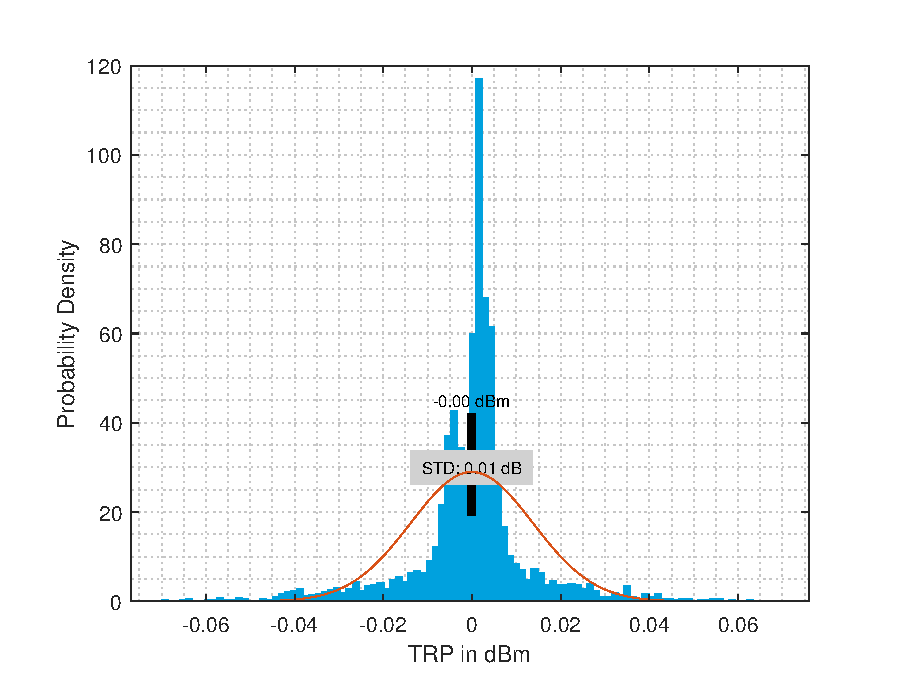
\includegraphics[width=0.49\textwidth]{Matlab/PDF_6-18_SF1.eps}}
  \centering
  \subfigure[CDF]{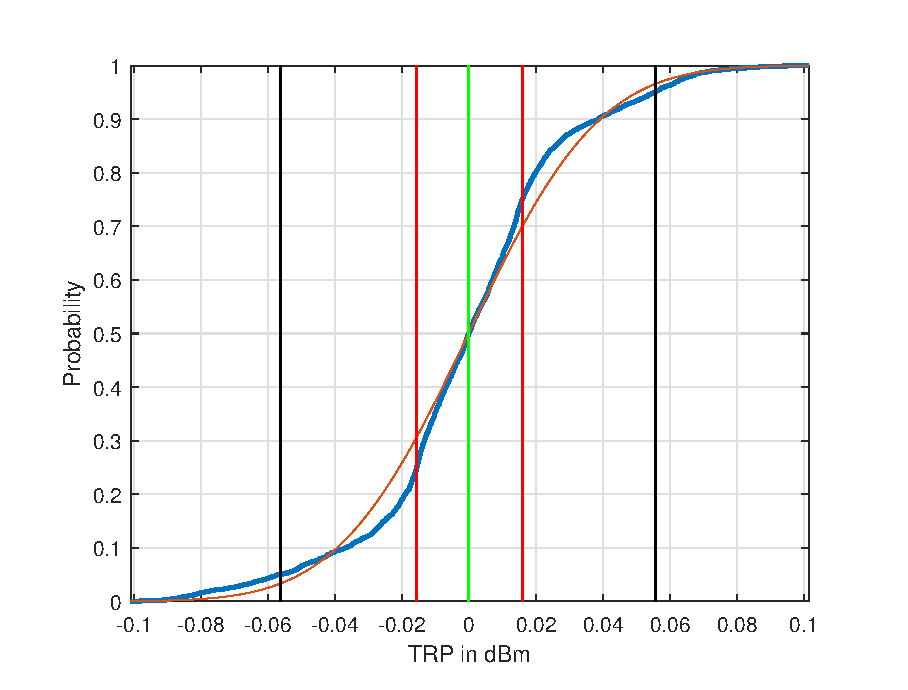
\includegraphics[width=0.49\textwidth]{{Matlab/CDF_6-18_SF1.eps}}}
\caption{4000 random steering vectors, $\text{SF}=1$, 6x18-Array}
\label{fig:rands}
\end{figure}

There are four input parameters first the \ac{SF}, second the \ac{CTF} and third and fourth the elements of the array in $y$ and $z$ direction. Every set of parameters is simulated with $N=4000$ samples. The azimuth steering is evenly distributed over the whole circle from $-\pi$ to $\pi$. In elevation a random variable is generated with a \ac{CDF} of \ac{CC} coefficients from $-\sfrac{\pi}{2}$ to $\sfrac{\pi}{2}$ by projecting evenly distributed random numbers. With that the main beam direction is evenly distributed over the spheres surface. For every set of parameters the third step is iterated $N$ times:

\begin{enumerate}
\item Generate $N$ steering vectors.
\item Derive a \ac{CSSG}.
\item Compute the \ac{TRP}:
\begin{enumerate}
\item Generate a antenna pattern using a random steering vector. A sample for that is depicted in figure \ref{fig:randp}.
\item Sample the antenna pattern with the derived grid.
\item Discard samples dependent on the \ac{CTF}.
\item Compute a \ac{TRP} using the \ac{CC}-quadrature.
\end{enumerate}
\end{enumerate}

A histogram and the resulting cumulative frequency diagram is plotted in figure \ref{fig:rands} (a) and (b). In both diagrams additionally the \ac{PDF}, respectively \ac{CDF} of the normal distribution is plotted in orange. Because the normal distribution is not a accurate metric for the underlying distribution, the $\SI{90}{\percent}$ \ac{IQR}, from the $\SI{5}{\percent}$ quantile to the $\SI{95}{\percent}$ quantile, is used to describe the scattering. In figure \ref{fig:rands} (b) the black lines are the $\SI{5}{\percent}$- and $\SI{95}{\percent}$- quantiles, the red lines the $\SI{25}{\percent}$- and $\SI{75}{\percent}$- quantiles and the mean is the green line.\\
The statistical experimental design is based on a D-optimal design dependent on the parameter matrix

\begin{equation}
X = \begin{bmatrix}
1 & \text{SF}_1 & \text{SF}_1^2 & \text{CTF}_1 & N_{y,1} & N_{z,1} & N_{y,1}N_{z,1}\\
\vdots & \vdots & \vdots & \vdots & \vdots & \vdots & \vdots\\
1 & \text{SF}_N & \text{SF}_N^2 & \text{CTF}_N & N_{y,N} & N_{z,N} & N_{y,N}N_{z,N}
\end{bmatrix}
\label{eq:parammatrix}
\end{equation}

with $M=7$ parameters. The D-optimal design is used because out of other documents e.q. \cite{2018arXiv180310993F} a course assumption to the significant parameters can be derived and thereby not every interaction needs to be tested. It is assumed that the \ac{SF} has also a quadratic dependency and that the linear interactions between the number of elements is also significant. With that a minimum number of samples is $N_\text{min}=1.5\cdot\left(M+1\right)=12$ \cite{dffs}. So a statistical experimental design can be derived using the Matlab\texttrademark{} \textit{cordexch(...)} with the input of the potency matrix of the regression

\begin{equation}
P = \begin{bmatrix}
0 & 0 & 0 & 0\\
1 & 0 & 0 & 0\\
2 & 0 & 0 & 0\\
0 & 1 & 0 & 0\\
0 & 0 & 1 & 0\\
0 & 0 & 0 & 1\\
0 & 0 & 1 & 1
\end{bmatrix},
\end{equation}

comparing the parameter matrix in equation \ref{eq:parammatrix}. With that the experimental design is derivable as 

\begin{equation}
X^\prime = \begin{bmatrix}
1&1&1&-1&1&-1&-1\\
1&1&1&1&-1&1&-1\\
1&1&1&1&-1&-1&1\\
1&0&0&-1&-1&-1&1\\
1&-1&1&-1&-1&-1&1\\
1&-1&1&-1&1&1&1\\
1&-1&1&1&-1&1&-1\\
1&-1&1&1&-1&-1&1\\
1&1&1&1&1&1&1\\
1&0&0&1&1&1&1\\
1&1&1&-1&1&1&1\\
1&-1&1&-1&-1&1&-1\\
1&0&0&-1&-1&1&-1\\
1&-1&1&1&1&-1&-1\\
1&1&1&-1&1&-1&-1\\
1&0&0&1&1&-1&-1
\end{bmatrix},
\end{equation}

where $1$ stands for the maximum value of the respective variable, analogue $-1$ for minimum and $0$ for middle. To generate a better regression and better possibilities of post processing a experimental design was generated sweeping every input parameter:

\begin{itemize}
\item The \ac{SF} is swept in the interval $\text{SF}=\left[0.5,2.5\right]$ using $25$ samples.
\item The \ac{CTF} is swept in the interval $\text{CTF}=\left[0,1\right]$ using $3$ samples with equal spacing.
\item The number of $y$ elements is swept in the interval $N_y=\left[2,14\right]$ using $4$ samples.
\item The number of $z$ elements is swept in the interval $N_z=\left[2,22\right]$ using $6$ samples.
\end{itemize}

This results in a experimental design with $N=25\cdot 3\cdot 4\cdot 6=1800$ samples. The total number of \ac{TRP} processions and pattern generations is thereby $N_\text{TRP}=1800\cdot 4000 = 7.200.000$, not including some reference samples to verify the computed regression.\\
Furthermore a comparison between \ac{CSSG} and \ac{CDG} shall be accomplished. Therefore the \ac{SF} needs to be projected on a \ac{CDG}. This is accomplished by computing the number of sampling points on the measurement sphere at $\text{CTF}=0$ and generating a \ac{CDG} with that number of points with the charged particle algorithm. The sampling is achieved by a $\SI{0.2}{\degree}$-\ac{CDG} and rounding the \ac{CDG} sample points to $k\cdot 0.2, k\in \mathbb{N}$. The quadrature to derive the \ac{TRP} is the mean of all samples.

\section{Result}

\begin{figure}
  \centering
  \subfigure[Scatter Plot]{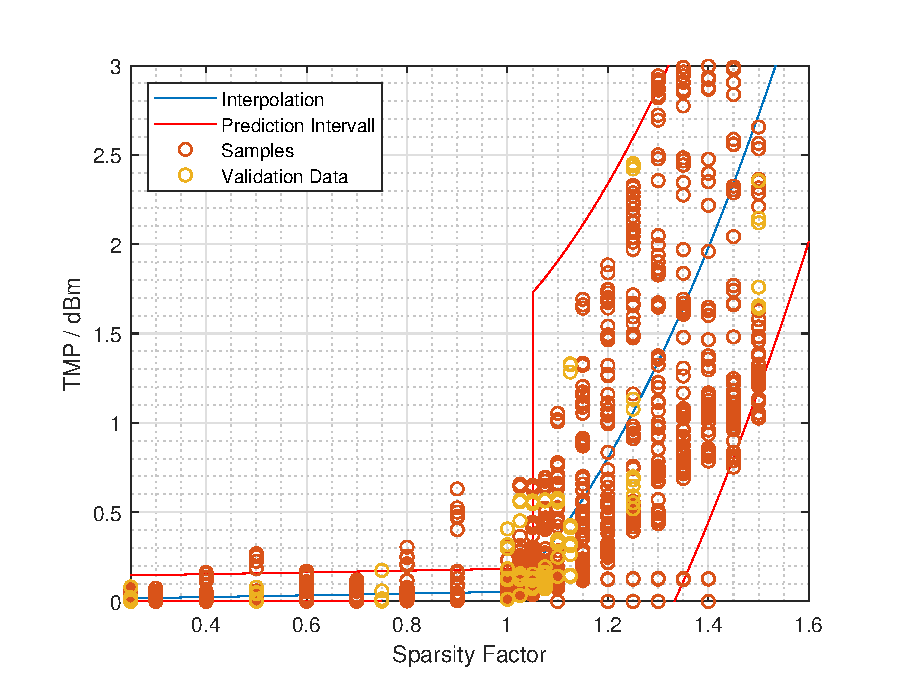
\includegraphics[width=0.49\textwidth]{Matlab/spars-sim1.eps}}
  \centering
  \subfigure[Box Plot]{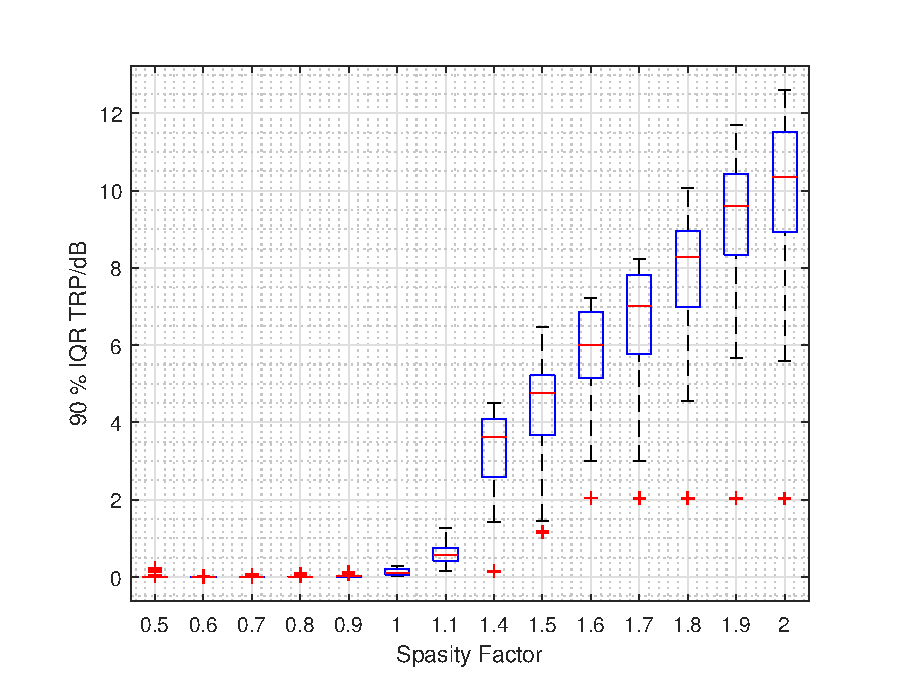
\includegraphics[width=0.49\textwidth]{{Matlab/spars-sim2.eps}}}
\caption{Simulation result over SF}
\label{fig:simressf}
\end{figure}

The marginal probability of the resulting \acp{TRP} from the simulation is depicted in figure \ref{fig:sparssim3}. There are two major areas, primarily the scattering of the \ac{TRP} is mostly independent from the \ac{SF}, secondary the \ac{TRP} is dependent from \ac{SF}. It seems that the \ac{TRP} is independent from all other input parameters.

\subsection{Regression}

The regression of the \ac{TRP} equation is done as described in section \ref{sec:regod} using the parameter matrix $X$ from equation \ref{eq:parammatrix}. The regression is carried out using the \textit{regstats(...)}-function by Matlab\texttrademark{}. Starting with this polynomial the \ac{CTF} is with a $p$-Value of $\SI{23}{\percent}$ not significant, the coefficient of determination is $\SI{77}{\percent}$. Discarding the \ac{CTF} and repeating the regression leads to also $\SI{77}{\percent}$ coefficient of determination and the constant term is not significant with a $p$-Value of $\SI{13}{\percent}$. The next discarded coefficient is the numbers of elements in $y$ with a  $p$-Value of $\SI{3.6}{\percent}$ leading to a coefficient of determination of $\SI{77}{\percent}$. Discarding the array size coefficients leads to a coefficient of determination of $\SI{55}{\percent}$. This could be caused by a small buck at the implementation of the simulation. For the \ac{CrefA} computing of the elevation angle increment, not the diameter of the array was taken but the maximum edge length, which leads to a slight dependency.\\
With the same approach the constant part is accounted. Also here a slight dependency from array size is found, discarding this leads to the combined function:

\begin{equation}
\text{TMP}\left(\text{SF}\right)=\begin{cases} -3.6\cdot\text{SF}+\frac{3.6}{\si{\decibel}}\cdot\text{SF}^2 & \text{for} SF>1.1\\
5.1\cdot 10^{-3}\si{\decibel}+4.9\cdot 10^{-2}\cdot \text{SF} & \text{for} SF\le 1.1\end{cases}
\end{equation}

and is plotted in figure \ref{fig:simressf} (a).

\subsection{CSSG vs. CDG}